

After mutual authentication and PIN entry, the charging terminal and ration card follow the communication protocol described in Figure \ref{figure:charging}. Charging terminal is also used to retrieve the logs and clear the memory of the smartcard. The logs constitute the non-repudiation evidence for any smartcard or terminal. Immediately after transferring the logs, the terminal verifies that the card is valid and that the balance is correct. Afterwards there are three different cases according to the result of the verification. An error means that the card must be revoked and the process ends. Otherwise, we distinct two cases for whether the card has been charged that month. 

\usetikzlibrary{matrix,shapes,arrows,positioning,chains, calc}

\begin{figure}[h!]

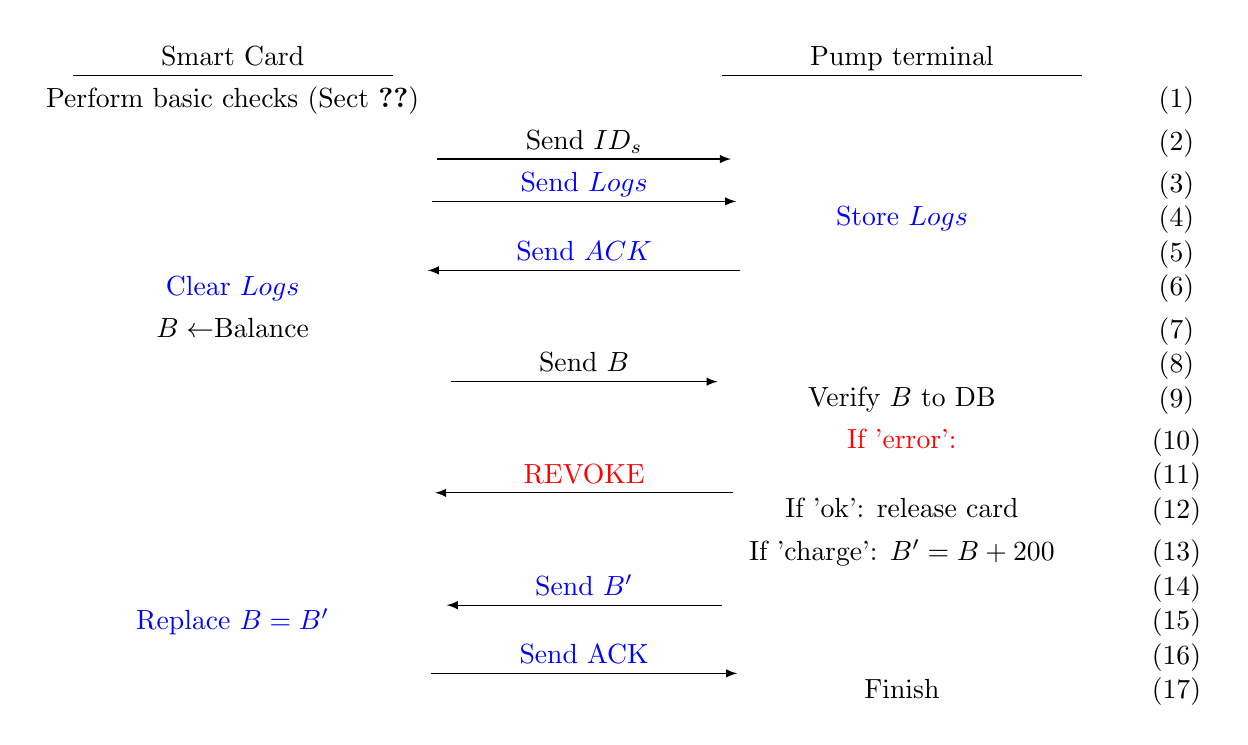
\begin{tikzpicture}
\matrix (m)[matrix of nodes, column  sep=1cm,row  sep=0.4mm, nodes={draw=none, anchor=center,text depth=0pt} ]{
Smart Card & & Pump terminal\\
Perform basic checks $($Sect \ref{section:lost}$)$ & & & $(1)$ \\
& Send $ID_{s}$ & & $(2)$ \\
\color{blue}&\color{blue} Send $Logs$ & & $(3)$ \\[-1mm]
\color{blue}&  &\color{blue} Store $Logs$ & $(4)$ \\[-1mm]
\color{blue}&\color{blue} Send $ACK$  & & $(5)$ \\[-1mm]
\color{blue} Clear $Logs$ &  &  & $(6)$ \\
$B\leftarrow$Balance & & & $(7)$ \\[-1mm]
& Send $B$ & & $(8)$ \\[-1mm]
& & Verify $B$ to DB & $(9)$ \\
\color{red}& &\color{red} If 'error': & $(10)$ \\[-1mm]
\color{red}&\color{red}REVOKE & & $(11)$ \\[-1mm]
& & If 'ok': release card & $(12)$ \\
& & If 'charge': $B'=B+200$ & $(13)$ \\[-1mm]
\color{blue}&\color{blue}Send $B'$ & & $(14)$ \\[-1mm]
\color{blue}Replace $B=B'$& & & $(15)$ \\[-1mm]
\color{blue}&\color{blue} Send ACK & & $(16)$ \\[-1mm]
& & Finish & $(17)$ \\[-1mm]
};

% Header
\draw[shorten <=-1cm,shorten >=-1cm] (m-1-1.south east)--(m-1-1.south west);
\draw[shorten <=-1cm,shorten >=-1cm] (m-1-3.south east)--(m-1-3.south west);

% Arrows
\draw[shorten <=-1cm,shorten >=-1cm,-latex] (m-3-2.south west)--(m-3-2.south east);
\draw[shorten <=-1cm,shorten >=-1cm,-latex] (m-4-2.south west)--(m-4-2.south east);
\draw[shorten <=-1cm,shorten >=-1cm,-latex] (m-6-2.south east)--(m-6-2.south west);
\draw[shorten <=-1cm,shorten >=-1cm,-latex] (m-9-2.south west)--(m-9-2.south east);
\draw[shorten <=-1cm,shorten >=-1cm,-latex] (m-12-2.south east)--(m-12-2.south west);
\draw[shorten <=-1cm,shorten >=-1cm,-latex] (m-15-2.south east)--(m-15-2.south west);
\draw[shorten <=-1cm,shorten >=-1cm,-latex] (m-17-2.south west)--(m-17-2.south east);

\end{tikzpicture}
\\Note: Steps 3 to 6 as well as 14 to 16 (in Blue) are atomic operations.
\caption{\label{figure:charging}Charging Terminal and Card communications}
\end{figure}

